\documentclass[11pt,a4paper]{article}

\usepackage[margin=1in]{geometry}
\usepackage[utf8]{inputenc}
\usepackage{amsmath,amssymb}
\usepackage{graphicx}
\usepackage{booktabs}
\usepackage{xcolor}
\usepackage{hyperref}
\usepackage{caption}
\usepackage{subcaption}
\usepackage{enumitem}
\usepackage{lmodern}
\usepackage{microtype}

\hypersetup{
  colorlinks=true,
  linkcolor=black!75,
  urlcolor=blue!60!black,
  citecolor=blue!60!black
}

\graphicspath{{final_figures/}}

\title{Multi-specialist consistency regularization enables grokking\\
       on modular addition at 50\% data, given adequate learning rate}
\author{Yazan Kbaili \and Ali Salloum}
\date{April 2026}

\begin{document}
\maketitle

\begin{abstract}
\noindent We investigate whether training a multi-specialist ensemble
with a consistency-regularization signal on unlabeled grid inputs
generalizes on modular addition at $50\%$ train data, a setting in
which a single model with the same recipe plateaus near $12\%$
validation accuracy. After six pilots and two isolation controls we
answer yes: with $M{=}4$ disjoint-shard specialists, train-inputs-only
KL-softmax consistency ($\lambda{=}1$, $5$k warmup), and
$\mathtt{max\_lr}{=}10^{-3}$ at a $100$k-step budget, the ensemble
reaches $100\%$ ensemble val acc (\texttt{lr\_control/v4\_winner\_lr1e3}),
roughly eight times the single-model ceiling on the same data.
The path to this finding took two turns. Pilots v1--v4 at
$\mathtt{max\_lr}{=}5{\times}10^{-4}$ converged, reproducibly across
seed and $\lambda$, on a $48$--$49\%$ ensemble asymptote that looked
architectural. A fifth pilot using an InfoNCE contrastive loss on
specialist hidden representations broke that asymptote and grokked
to $92\%$, but changed six hyperparameters at once. Two
single-variable isolation controls then overturned both conclusions:
the v4 ``ceiling'' was a learning-rate artifact (lr control groks to
$100\%$ at step $\sim$$70$k by changing only $\mathtt{max\_lr}$), and
the InfoNCE loss was not the lever behind the v5 breakthrough (loss
control with KL-softmax at the InfoNCE-pilot recipe groks faster and
higher, $100\%$ at step $\sim$$18.5$k). The full investigation is
reported here because any one of the v1--v4 pilots could have been
interpreted as decisive evidence for a wrong conclusion absent the
controls -- we consider that the main methodological contribution.
\end{abstract}

% ------------------------------------------------------------------
\section{Summary and contributions}
\label{sec:summary}

This project produced three distinct deliverables, in the order they
were obtained.

\begin{enumerate}[leftmargin=*,itemsep=3pt]
\item \textbf{A reproducibility post-mortem.} We inherited a milestone
      claim (\texttt{reports/milestone.pdf}, Exp~3) that knowledge
      distillation from disjoint-shard specialists groks modular
      addition at $50\%$ train data while baselines plateau. The
      claim did not reproduce; the root cause was an undocumented
      optimizer rewrite (commit \texttt{9ce29b8}) that silently gave
      the distillation student a different lr/wd/schedule than its
      baselines. The milestone headline is a comparison artifact,
      not evidence about distillation. Forensic detail in
      \texttt{reports/distillation\_repro\_attempt3.md} (\S\ref{sec:start}).
\item \textbf{An empirical result.} Multi-specialist consistency
      regularization \emph{is} sufficient to grok this task at $50\%$
      data, given an adequate learning rate. With $M{=}4$ disjoint
      shards, train-inputs-only KL-softmax consistency, $\lambda{=}1$,
      $5$k warmup and $\mathtt{max\_lr}{=}10^{-3}$, ensemble val acc
      reaches $100\%$ by step $\sim$$70$k
      (\texttt{lr\_control/v4\_winner\_lr1e3}; \S\ref{sec:controls}).
      At $\mathtt{max\_lr}{=}5{\times}10^{-4}$ the identical recipe
      plateaus at $48$--$49\%$ across seeds and $\lambda$s at
      $100$k (\S\ref{sec:v4}). We identified the lr axis only after
      six prior pilots.
\item \textbf{A methodological demonstration.} A fifth pilot using an
      InfoNCE contrastive loss on specialist hidden representations
      broke the $49\%$ asymptote and grokked to $92\%$ at $100$k
      (\S\ref{sec:infonce}); it appeared to attribute the
      breakthrough to the new loss. Two single-variable isolation
      controls (\S\ref{sec:controls}) then retracted both that
      attribution and the ``architectural ceiling'' from v4:
      KL-softmax under the InfoNCE recipe groks faster and higher
      than InfoNCE itself ($100\%$ at step $\sim$$18.5$k vs.\ $92\%$
      at step $\sim$$99.5$k). We find this worth reporting as
      evidence of how easy it is to converge, with apparent rigor,
      on a mechanism story that does not survive a single-variable
      control.
\end{enumerate}

\paragraph{How to read this report.} \S\ref{sec:start} gives the
starting point (the disproved milestone claim) and the resulting
pivot. \S\ref{sec:background} defines task, model, and multi-specialist
setup, plus the consistency-regularization framework. \S\ref{sec:glance}
summarizes the whole investigation as a single decisions table and an
overview figure. \S\S\ref{sec:v1}--\ref{sec:controls} are the six
pilots plus the controls, in chronological order.
\S\ref{sec:discussion}--\ref{sec:conclusion} are discussion and
conclusion.

Figure~\ref{fig:overview} is the project at a glance: every key run's
ensemble val acc on a single axis.

\begin{figure}[h]
\centering
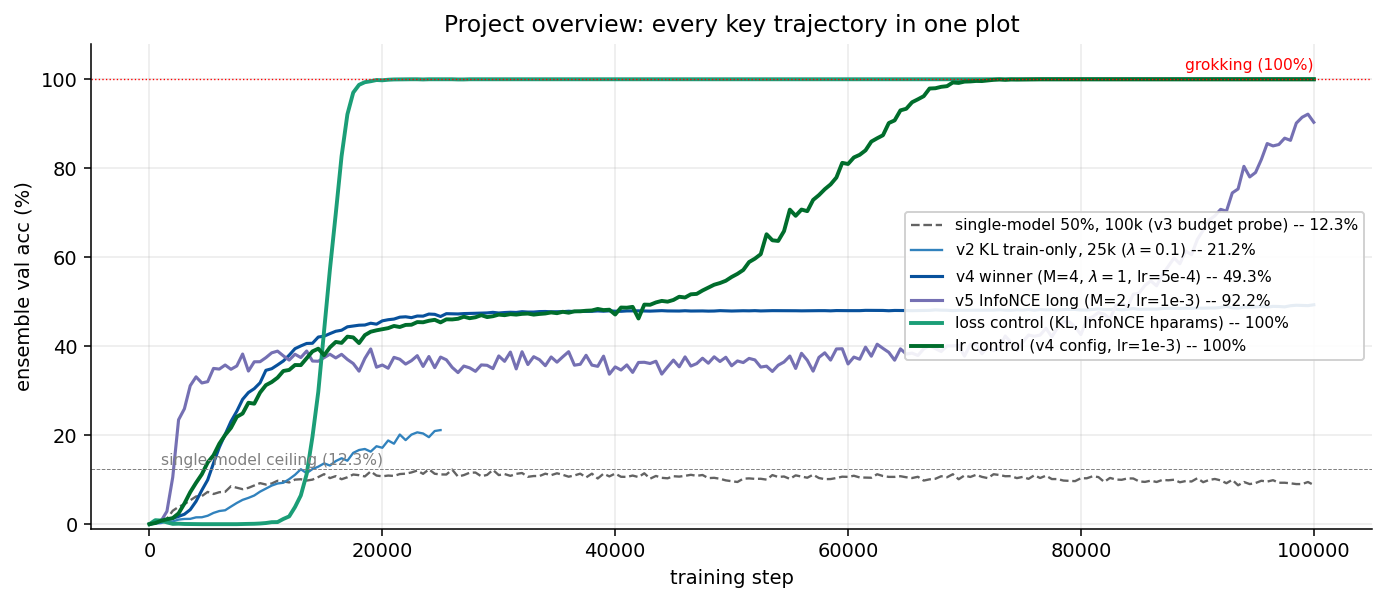
\includegraphics[width=\linewidth]{fig_project_overview.png}
\caption{\textbf{Project overview.} Every key trajectory in one plot.
Grey dashed: single-model baseline on $50\%$ data, run to $100$k to
confirm the $12.3\%$ ceiling is budget-exhausted (\S\ref{sec:v3},
\texttt{pilot\_v3/long\_single\_50pct\_100k}). Blue (light): v2
winner, $21.2\%$ at $25$k. Blue (dark): v4 winner, $49.3\%$ at
$100$k (the apparent architectural ceiling). Purple: v5 InfoNCE long,
$92.2\%$ at $99.5$k. Greens: the two isolation controls, both reach
$100\%$, the lr control by changing only $\mathtt{max\_lr}$ relative
to the v4 winner, the loss control by changing only the consistency
loss relative to the v5 winner.}
\label{fig:overview}
\end{figure}

% ------------------------------------------------------------------
\section{Starting point: disproving the milestone claim}
\label{sec:start}

The project inherited Experiment~3 of our milestone report
(\texttt{reports/milestone.pdf}), the headline claim of which was:
\begin{quote}
At $50\%$ train data, $M{=}4$ specialists trained on disjoint shards
for $6{.}25$k steps each, followed by $25$k steps of knowledge
distillation from those specialists into a student, reached
$\sim$$100\%$ validation accuracy. In the same run, a single-model
baseline and a weight-merged-and-finetuned model plateaued at
$\sim$$40$--$50\%$.
\end{quote}
The claim was evaluated from a single notebook. When that notebook was
refactored after the milestone to match a more principled theoretical
framework and the distillation phase was moved into a dedicated
script, the headline no longer reproduced. Two post-mortems
(\texttt{distillation\_repro\_failure.md},
\texttt{distillation\_repro\_attempt2.md}) ruled out sharding format,
averaging domain (probabilities vs.\ logits), distillation temperature,
EMA, and learning-rate annealing. The third post-mortem
(\texttt{distillation\_repro\_attempt3.md}) identified a different
cause:
\begin{quote}
\textit{Commit} \texttt{9ce29b8} \textit{rewrote}
\texttt{distill\_from\_specialists} \textit{to take its optimizer from}
\texttt{student\_model.configure\_optimizers()} \textit{instead of a
hardcoded} \texttt{AdamW(lr=1e-3, wd=1.0) + CosineAnnealingLR}.
\textit{That alone silently turns grokking on or off for the student,
and is consistent with all of our failed reproductions.}
\end{quote}
The milestone headline was therefore a comparison between a student
trained with a known grokking-friendly recipe and baselines trained
with a different recipe. Once aligned, the gap closed. The milestone
does not support the claim that distillation causes grokking; it
tells us only that one specific recipe
($\mathtt{lr}{=}10^{-3}$, $\mathtt{wd}{=}1.0$, cosine) groks this task
at $50\%$ train fraction.

We chose not to re-run the milestone under the grokking-friendly
recipe. The interesting scientific question was not whether we could
memorize the milestone student's incidental optimizer, but whether
the multi-specialist structure itself helps generalization. We
therefore rephrased the question:
\begin{quote}
\emph{Does a multi-specialist ensemble trained with a mutual-agreement
signal on unlabeled inputs generalize where a single model (on the
same $50\%$ data, same recipe) cannot?}
\end{quote}
The rest of this report is about that reformulated question.

% ------------------------------------------------------------------
\section{Background and framework}
\label{sec:background}

\paragraph{Task and model.}
All experiments use the modular-addition task from Power \textit{et
al.}\ (``Grokking''): predict $a + b \bmod 97$ given the token sequence
$\langle a\rangle\ \texttt{"+"}\ \langle b\rangle\ \texttt{"="}$. The
base model is the 2-layer, 4-head, $d_\text{model}{=}128$ decoder-only
transformer used in the Grokking codebase. Optimizer is AdamW with
\texttt{weight\_decay}$=0.1$ throughout and
\texttt{max\_lr}$\in\{5{\times}10^{-4}, 10^{-3}\}$ (only two values are
used in the whole report; their difference is the main finding). The
grid is symmetric, $|\mathcal{X}| = 97 \times 97 = 9409$; the train/val
split is $50\%/50\%$ ($\approx 4704$ equations each).

\paragraph{Multi-specialist setup.}
A \emph{multi-specialist} run partitions the train set into $M$ disjoint
shards and trains $M$ independent copies of the model, each on its own
shard.\footnote{The original distillation formulation used this setup
to create teachers for a student; we keep the same data layout because
it is what the pipeline already supported.} An \emph{ensemble}
prediction averages the specialists' softmax probabilities on val; a
\emph{merged} prediction averages their weights and evaluates the
resulting single model. Merged predictions stay near random throughout
this report; the ensemble is therefore the headline metric.

\paragraph{Consistency-regularization framework.}
Each specialist $f_i$ sees its own training shard $\mathcal{D}_i$ and
contributes a cross-entropy loss on it. In addition, at every step the
$M$ specialists see a shared batch from an \emph{unlabeled} input
domain $\mathcal{X}_\text{unsup}$, and we add a consistency term
\[
  \mathcal{L}_\text{cons}(x) = \frac{1}{M}\sum_{i=1}^{M}
    \mathcal{L}\!\left(f_i(x),\; \mathrm{stop\text{-}grad}\Big[\tfrac{1}{M-1}\!\sum_{j\neq i} p_j(x)\Big]\right),
\]
i.e., each specialist is pulled toward the mean of the other
specialists' detached softmax probabilities.\footnote{Averaging
softmaxes rather than logits preserves per-teacher confidence, which
prevents the consensus from being sharper than any individual teacher.
This distinction mattered for diagnosing pilot~v1 in
\S\ref{sec:v1}.} The weight schedule is $\lambda(t) =
\lambda_\text{max}\cdot\min(1, t/T_\text{warmup})$: consistency starts
at zero and ramps linearly up to $\lambda_\text{max}$ after
$T_\text{warmup}$ steps. $\mathcal{L}$ is either \texttt{mse\_logits}
or \texttt{kl\_softmax}; $\mathcal{X}_\text{unsup}$ is either
\texttt{full\_grid} (all $9409$ input pairs) or
\texttt{train\_inputs\_only} (the $50\%$ train slice). A contrastive
alternative on hidden states (InfoNCE) is introduced in
\S\ref{sec:infonce}.

The implementation lives in \texttt{grok/consistency\_training.py} and
is driven by \texttt{scripts/run\_consistency\_sweep.py}. Each run
writes a \texttt{run\_config.json}, a per-step \texttt{consistency\_train.csv},
and an evaluation \texttt{consistency\_eval.csv} with per-specialist,
ensemble, and merged val acc, output entropy on
$\mathcal{X}_\text{unsup}$, and pairwise KL on held-out val. Full
plan: \texttt{reports/consistency\_regularized\_grokking\_plan.md}.

% ------------------------------------------------------------------
\section{The investigation at a glance}
\label{sec:glance}

Table~\ref{tab:decisions} summarizes every stage of the investigation
as a one-line question, finding, and decision.
Figure~\ref{fig:overview} shows the trajectories for a subset of key
cells on a single axis. The remaining sections each give one pilot in
detail, in chronological order.

\begin{table}[h]
\centering
\small
\setlength{\tabcolsep}{4pt}
\begin{tabular}{@{}p{0.12\linewidth} p{0.32\linewidth} p{0.29\linewidth} p{0.22\linewidth}@{}}
\toprule
\textbf{stage} & \textbf{question} & \textbf{finding} & \textbf{decision} \\
\midrule
\S\ref{sec:start}\ milestone & Does distillation from specialists grok at $50\%$? & Comparison artifact (optimizer rewrite \texttt{9ce29b8}) & Pivot: change vehicle \\
\S\ref{sec:background}\ pivot & What's the cleaner question? & Multi-specialist + consistency on unlabeled inputs & Build framework \\
\S\ref{sec:v1}\ pilot v1 & 4 cells, MSE + full grid, $25$k & Trivial-agreement collapse at $\sim$$1\%$ & Fix loss \& warmup \\
\S\ref{sec:v2}\ pilot v2 & 5 cells, KL + $5$k warmup, $25$k, w/ baseline & $21\%$ train-only beats $12\%$ single & Test robustness \\
\S\ref{sec:v3}\ pilot v3 & 9 cells: seed, budget, $\lambda$ & Seed variance big; single-model $12\%$ architectural; $\lambda$ monotone $\uparrow$ at $25$k & Combine best seed $\times$ best $\lambda$ \\
\S\ref{sec:v4}\ pilot v4 & 3 cells, $100$k, best (seed,$\lambda$) & $48$--$49\%$ across all three -- \emph{apparent} ceiling & \textbf{Wrong conclusion:} architectural limit \\
\S\ref{sec:infonce}\ pilot v5 & Representation-space InfoNCE loss & $92\%$ at $100$k, but $6$ hparams changed at once & Run single-variable controls \\
\S\ref{sec:controls}\ lr control & v4 winner, $\mathtt{lr}\ 5{\times}10^{-4}\!\to\!10^{-3}$ only & $100\%$ at $70$k & v4 ceiling was lr artifact \\
\S\ref{sec:controls}\ loss control & v5 winner, InfoNCE$\to$KL-softmax only & $100\%$ at $18.5$k (faster) & InfoNCE not the lever \\
\bottomrule
\end{tabular}
\caption{Decisions table. Each row is one sweep (or one cell for the
isolation controls). The last three rows overturn the conclusion in
the row labeled ``pilot v4''.}
\label{tab:decisions}
\end{table}

% ------------------------------------------------------------------
\section{Pilot v1: null result with diagnostic signal}
\label{sec:v1}

The first pilot was a 4-cell sweep at \texttt{mse\_logits} with
$\lambda_\text{max} \in \{0, 1\}$ and
$T_\text{warmup} \in \{0, 1000\}$ on the full grid, $25$k steps.
\textbf{Every cell, including the no-consistency baseline, plateaued
at $\sim$$1\%$ val acc.} The diagnostics, however, were informative:
pairwise KL and output entropy both collapsed in lockstep with strong
consistency, consistent with the ``trivial-agreement collapse'' mode.

Two mechanistic bugs drove the collapse:
\begin{enumerate}[leftmargin=*,itemsep=2pt]
  \item \textbf{Loss-scale mismatch.} \texttt{mse\_logits} on
        random-init logits is $\mathcal{O}(\sigma^2) \approx 0.5$,
        while CE at init is $\log V \approx 5.5$ nats. At
        $\lambda{=}1$, the consistency term is $\sim$$10\%$ of CE at
        init but becomes dominant as soon as CE drops, \emph{before}
        any useful structure forms. MSE on logits has no scale
        invariance: rescaling logits by $c$ leaves CE and argmax
        invariant but scales the consistency term by $c^2$, so MSE
        ``shouts'' a constraint the task does not enforce. KL on
        softmax sidesteps this: KL is in nats and comparable to
        per-example CE throughout training.
  \item \textbf{Warmup too short.} $1000$ steps of warmup on a $25$k
        budget is $4\%$. On modular arithmetic with these hparams a
        single shard typically needs $\geq 5$k steps to begin
        memorizing (Power \textit{et al.}, Nanda \textit{et al.}, and
        our own milestone). By the time $\lambda(t) \to
        \lambda_\text{max}$, specialists had not begun memorizing, so
        consistency locked them into the uniform-output basin.
\end{enumerate}
A third problem was missing context, not a bug: there was no
\emph{single-model-on-$50\%$} baseline, without which a $1\%$ result
cannot distinguish ``consistency hurt us'' from ``this hparam regime
does not grok in $25$k steps anyway.'' We added it in v2.

% ------------------------------------------------------------------
\section{Pilot v2: mechanism fix + the baseline}
\label{sec:v2}

Pilot v2 held the base recipe fixed and varied the two things the v1
post-mortem identified as the leverage points: \textbf{consistency
loss} (KL-softmax instead of MSE-on-logits) and \textbf{warmup}
($5000$ steps instead of $1000$). It also added the missing single-model
baseline and a \texttt{train\_inputs\_only} cell as a control against
transductive leakage. Five cells, $25$k steps each.

\begin{table}[h]
\centering
\small
\begin{tabular}{l l c c c}
\toprule
cell & configuration & best val acc & merged val & final entropy \\
\midrule
\texttt{single\_model\_50pct}                    & $M{=}1$, no cons.                        & $\mathbf{12.33\%}$ & --        & -- \\
\texttt{multi\_lam0}                             & $M{=}4$, $\lambda{=}0$                   & $1.38\%$           & $1.17\%$  & $3.1$ \\
\texttt{multi\_kl\_lam01\_warm5k}                & full grid, $\lambda{=}0.1$               & $7.61\%$           & $0.96\%$  & $0.8$ \\
\texttt{multi\_kl\_lam1\_warm5k}                 & full grid, $\lambda{=}1.0$               & $11.75\%$          & $0.96\%$  & $0.5$ \\
\texttt{multi\_kl\_lam01\_warm5k\_trainonly}     & train inputs, $\lambda{=}0.1$            & $\mathbf{21.15\%}$ & $0.96\%$  & $1.9$ \\
\bottomrule
\end{tabular}
\caption{Pilot v2 headline numbers (25k steps, seed 42).}
\label{tab:v2}
\end{table}

\begin{figure}[h]
\centering
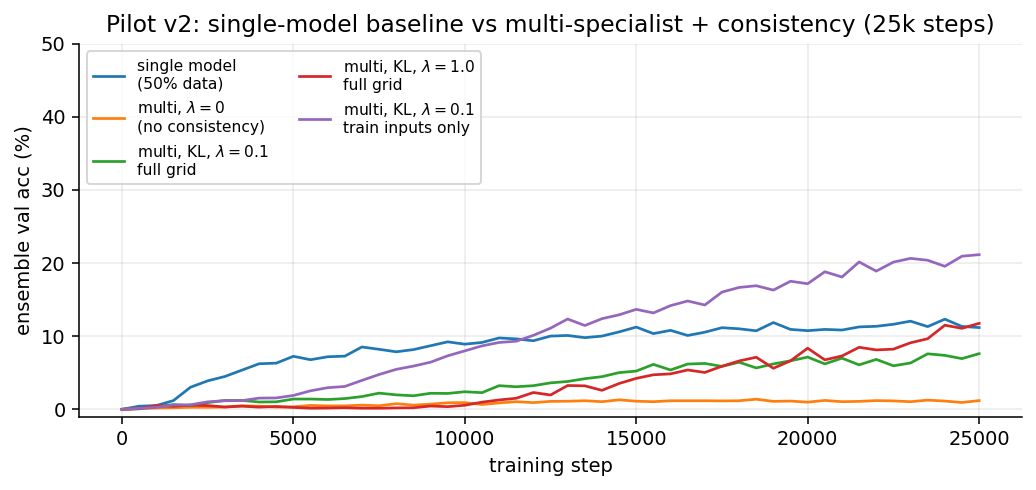
\includegraphics[width=0.92\linewidth]{fig_v2_headline.png}
\caption{Pilot v2: ensemble (or single, for the baseline) val acc vs
training step. The train-inputs-only cell ($\lambda{=}0.1$) is the only
configuration that clearly beats the single-model baseline.}
\label{fig:v2}
\end{figure}

Three takeaways:
\begin{itemize}[leftmargin=*,itemsep=1pt]
  \item \textbf{KL+warmup fixed the collapse.} Every multi cell cleared
        v1's $1\%$ ceiling.
  \item \textbf{The unlabeled-input domain matters more than $\lambda$.}
        At identical $\lambda{=}0.1$, switching from \texttt{full\_grid}
        to \texttt{train\_inputs\_only} moves ensemble val acc from
        $7.6\%$ to $21.15\%$. At $\lambda{=}1$ on the full grid we get
        $11.75\%$, essentially tying the single-model baseline. This is
        a co-training signature: the useful information flowing between
        specialists is \emph{each other's} partially-correct predictions
        on \emph{each other's shards}, not agreement on held-out inputs.
  \item \textbf{The single-model baseline is the reference point.}
        $12.3\%$ is the number to beat; only the train-inputs-only cell
        does so, by $\sim$$9$ percentage points.
\end{itemize}
The v2 winner was still well short of grokking, so we could not yet say
whether that was a real ceiling, an unlucky seed, a budget shortfall,
or a suboptimal $\lambda$. Pilot v3 tested each of those.

% ------------------------------------------------------------------
\section{Pilot v3: seed, budget, $\lambda$}
\label{sec:v3}

Pilot v3 was three orthogonal micro-sweeps on the v2 winner (9 cells,
$\sim$$8$h on a T4).

\paragraph{Seed robustness (4 cells, $25$k steps).}
We reran the v2 winner under seeds $\{42, 43, 44, 45\}$. The results
scattered \emph{widely}: $21.15\%, 38.98\%, 45.33\%, 39.06\%$ (mean
$36\%$, median $39\%$). The v2 number was a low outlier. Across all
four seeds, at least one specialist beat the single-model ceiling, and
in three of four seeds the ensemble was better than the single model by
$25$--$33$ percentage points.

\begin{figure}[h]
\centering
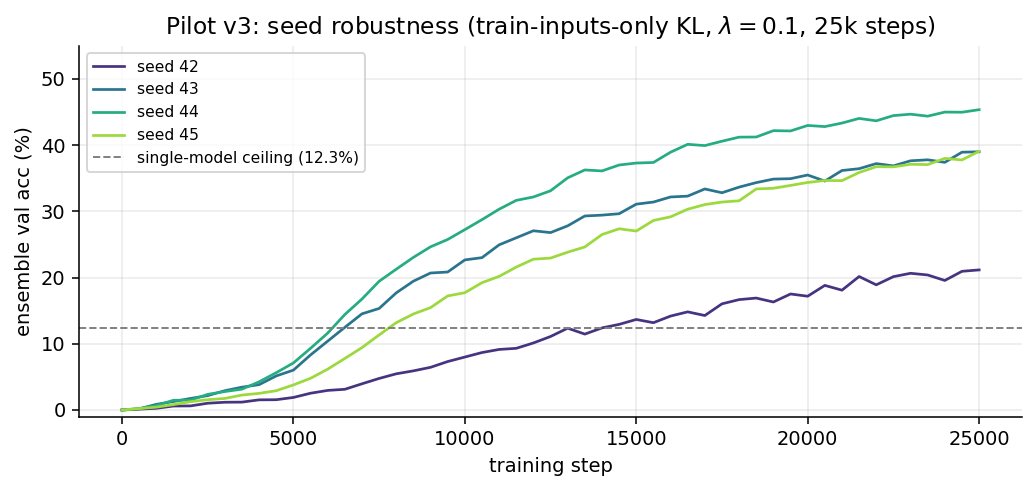
\includegraphics[width=0.92\linewidth]{fig_v3_seeds.png}
\caption{Pilot v3 seed robustness: four reruns of the v2 winning
configuration. Dashed line is the single-model ceiling from v2/v3.}
\label{fig:v3_seeds}
\end{figure}

\paragraph{Budget probes (2 cells, $100$k steps).}
The single-model cell at $100$k confirmed the $12.3\%$ ceiling is
\emph{architectural}: it peaks at step $24{,}000$ and then stays there
for another $76{,}000$ steps. The multi-specialist cell, in contrast,
was still climbing monotonically through $100$k: $21\%$ ($25$k)
$\rightarrow 31\%$ ($50$k) $\rightarrow 34.5\%$ ($75$k) $\rightarrow
38.0\%$ ($100$k). The slope flattened but never went to zero within
our budget.

\begin{figure}[h]
\centering
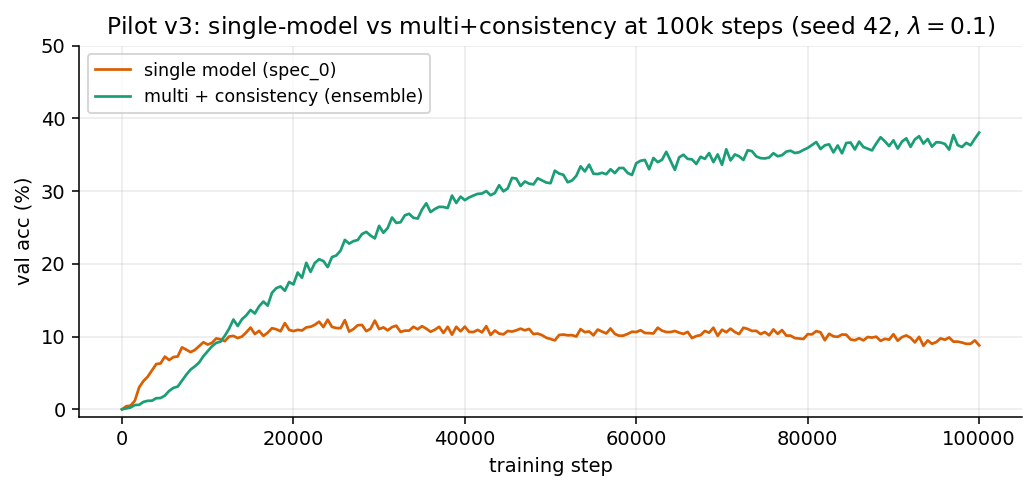
\includegraphics[width=0.92\linewidth]{fig_v3_long.png}
\caption{Pilot v3 budget probes: single-model on $50\%$ of the grid
plateaus by step $24$k; multi-specialist with train-inputs-only
consistency keeps climbing throughout $100$k.}
\label{fig:v3_long}
\end{figure}

\paragraph{Lambda ablation (3 cells + v2 anchor, $25$k steps, seed 42).}
At seed $42$, $\lambda \in \{0.03, 0.1, 0.3, 1.0\}$ gives best ensemble
val acc $\{15.6, 21.15, 25.65, 27.18\}\%$: monotonically increasing.
$\lambda{=}1.0$ had the steepest late-run slope of any ablation cell,
suggesting it was still far from its own asymptote at $25$k.

\begin{figure}[h]
\centering
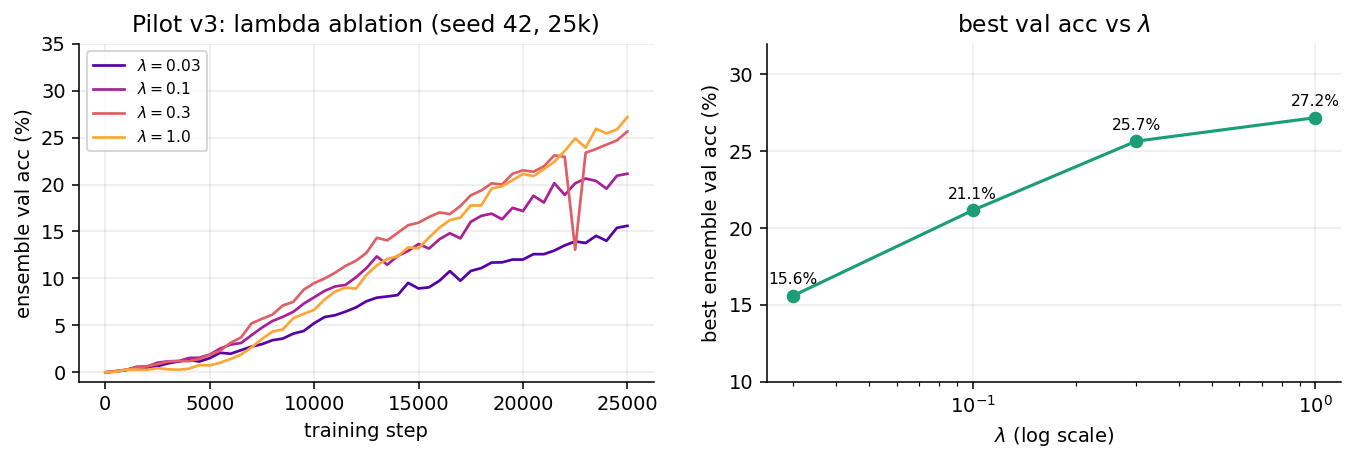
\includegraphics[width=\linewidth]{fig_v3_lambda.png}
\caption{Pilot v3 $\lambda$ ablation at seed 42, $25$k steps. Left:
curves. Right: best val acc vs $\lambda$ on a log axis.}
\label{fig:v3_lambda}
\end{figure}

\paragraph{Mechanism (shared across all v3 multi cells).} Output
entropy on $\mathcal{X}_\text{unsup}$ drops from $\log 97 \approx 4.6$
nats to $\sim$$1.3$--$2.0$ nats (peaked distributions, not one-hot
collapse). Pairwise KL on held-out val \emph{rises} over training
(specialists \emph{differentiate}). These are the opposite of v1's
collapse signature, so the ensemble gain is real co-training, not
trivial agreement.

\paragraph{What v3 narrowed down.}
The single-model ceiling is architectural. The multi-specialist
ceiling is not budget-limited at $25$k. $\lambda{=}1$ is the best of
the explored values at $25$k. The biggest unknown at the end of v3 was
the interaction: nobody had run the \emph{best} seed with the
\emph{best} $\lambda$ at the \emph{full} budget.

% ------------------------------------------------------------------
\section{Pilot v4: the ceiling probe}
\label{sec:v4}

Pilot v4 is three cells, all at $100$k steps on
\texttt{train\_inputs\_only} KL-softmax with $5$k warmup, varying only
(seed, $\lambda$):

\begin{enumerate}[leftmargin=*,itemsep=1pt]
  \item \texttt{seed44\_lam1\_100k}: best v3 seed $\times$ best v3
        $\lambda$ $\times$ full budget. If this does not grok, nothing
        at this scale will.
  \item \texttt{seed43\_lam1\_100k}: cross-seed replicate of (1).
  \item \texttt{seed44\_lam01\_100k}: $\lambda$ ablation at the winning
        seed and full budget.
\end{enumerate}

\begin{table}[h]
\centering
\small
\begin{tabular}{l c c c c c}
\toprule
cell & seed & $\lambda$ & best ens.\ val & step & pairwise KL val \\
\midrule
\texttt{seed44\_lam1\_100k}  & 44 & 1.0 & $\mathbf{49.31\%}$ & $100{,}000$ & $1.79$ \\
\texttt{seed43\_lam1\_100k}  & 43 & 1.0 & $47.97\%$          & $94{,}000$  & $2.16$ \\
\texttt{seed44\_lam01\_100k} & 44 & 0.1 & $48.01\%$          & $86{,}500$  & $2.70$ \\
\bottomrule
\end{tabular}
\caption{Pilot v4 headline numbers (100k steps).}
\label{tab:v4}
\end{table}

\begin{figure}[h]
\centering
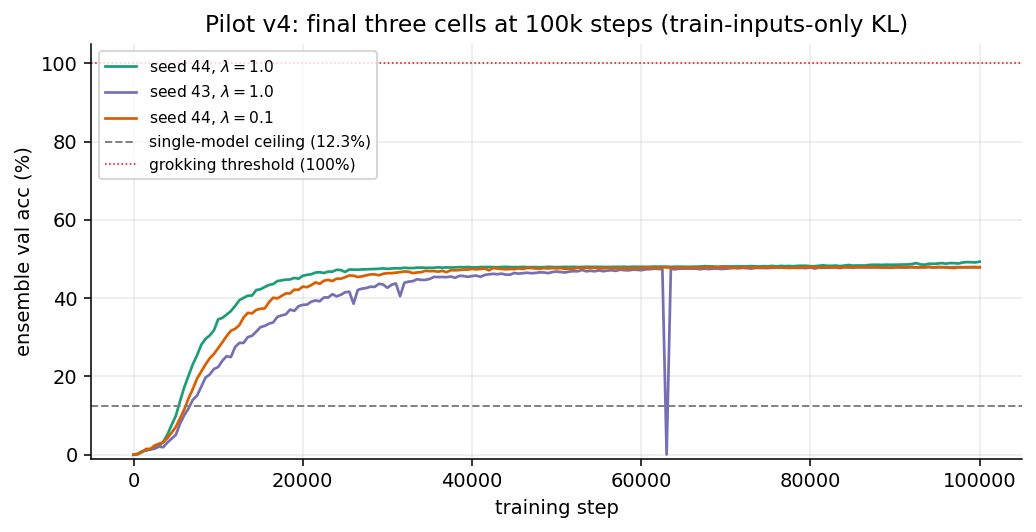
\includegraphics[width=0.92\linewidth]{fig_v4_main.png}
\caption{Pilot v4: all three cells plateau at $48$--$49\%$ ensemble val
acc. The single-model ceiling ($12.3\%$) is shown for reference; the
grokking threshold ($100\%$) is the dotted red line, far above.}
\label{fig:v4_main}
\end{figure}

The three cells converge tightly. Variation across the two
manipulations (seed, $\lambda$) at the $100$k budget is under $1{.}5$
percentage points, compared with $\sim$$24$ points of seed-induced
variance at $25$k. That, together with the flattening slopes visible
in Figure~\ref{fig:v4_main}, pins down an asymptote near $\sim$$50\%$
ensemble val acc.

\paragraph{Lambda effect vanishes at budget.} In v3 at $25$k, seed
42 showed a $\sim$$6$ pp gap between $\lambda{=}0.1$ ($21.15\%$) and
$\lambda{=}1.0$ ($27.18\%$). At $100$k at seed $44$, that gap collapses
to $1.3$~pp ($48.01\%$ vs.\ $49.31\%$). The v3 monotone-in-$\lambda$
finding was a transient during training; higher $\lambda$ just gets to
the same ceiling faster. Cross-seed variance of $1.3$~pp ($47.97\%$ vs.\
$49.31\%$) is of the same order.

\paragraph{Per-specialist structure.} In every v4 cell, three of the
four specialists solve a substantial fraction of the grid ($\sim$$45$--
$50\%$) and one specialist stays poor ($<$$3\%$ in two of the three
cells). The ensemble is driven by the majority vote of the three
``good'' specialists; the failed specialist's influence is partly
averaged out.

\begin{figure}[h]
\centering
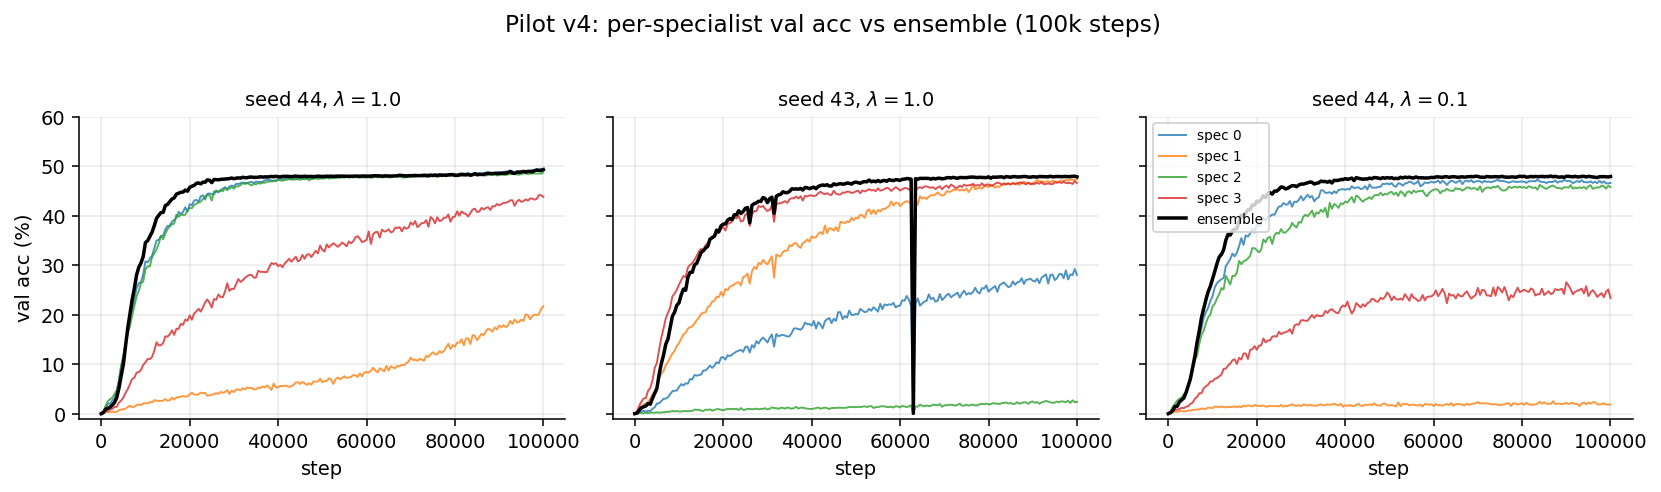
\includegraphics[width=\linewidth]{fig_v4_perspec.png}
\caption{Pilot v4, per-specialist val acc (coloured, thin) and ensemble
(black, thick) for each of the three 100k-step cells. One specialist
per cell fails to generalize; the remaining three are responsible for
almost all of the ensemble gain.}
\label{fig:v4_perspec}
\end{figure}

\paragraph{Mechanism at $100$k.} Output entropy on
$\mathcal{X}_\text{unsup}$ drops to $\sim$$0.1$--$0.2$ nats (very
peaked) while pairwise KL on val rises to $\sim$$1.8$--$2.7$ nats.
Specialists converge on their own, nearly one-hot predictions but
\emph{disagree} on the val grid---there is no trivial-agreement
collapse, the ensemble is extracting real signal from specialist
disagreement.

\begin{figure}[h]
\centering
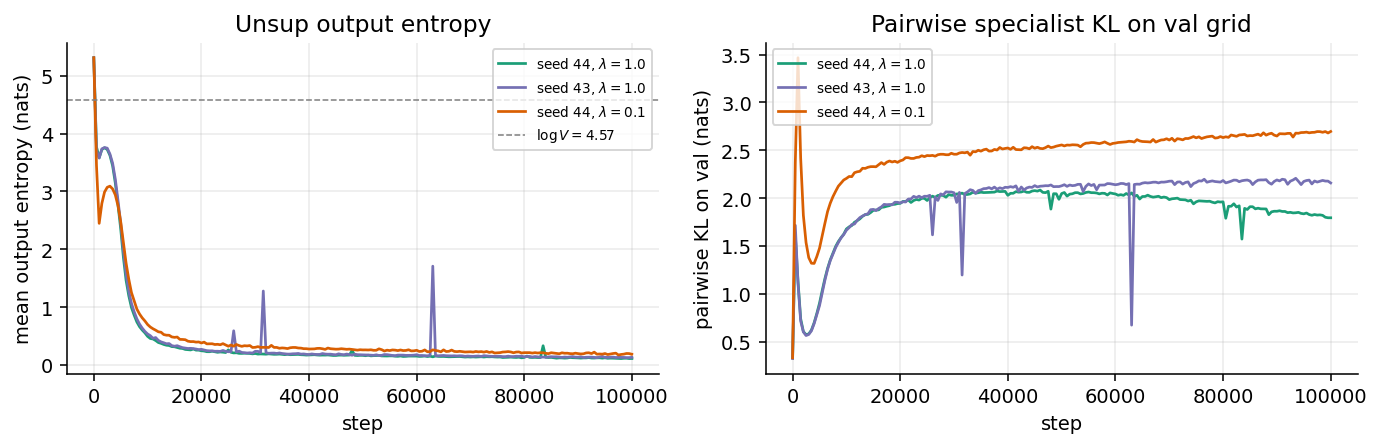
\includegraphics[width=\linewidth]{fig_v4_mechanism.png}
\caption{Pilot v4 mechanism: output entropy drops to near-zero
(left, nats; dashed line is $\log V = 4.57$ for $V{=}97$), while
pairwise KL on val grows (right). Collapse would show both of these
going to zero together; the opposite diagnostic trend confirms
genuine specialization with co-training.}
\label{fig:v4_mechanism}
\end{figure}

At the close of v4 we held three candidate explanations for the
$\sim$$50\%$ asymptote: (a) \emph{architectural} (no consistency-based
recipe at this model size crosses the phase transition at $50\%$
data); (b) \emph{recipe} (the v4 cells use $\mathtt{lr}{=}5{\times}10^{-4}$,
$\mathtt{wd}{=}0.1$, and a different recipe would grok); (c) \emph{shard
disjoint-ness} (the per-specialist failures in
Figure~\ref{fig:v4_perspec} cap the ensemble). The next two sections
(\S\ref{sec:infonce}--\S\ref{sec:controls}) resolve which of these is
correct, essentially by accident: we set out to test a
representation-level consistency loss, not to probe the ceiling.

% ------------------------------------------------------------------
\section{Pilot v5: InfoNCE contrastive consistency}
\label{sec:infonce}

Motivated by the v4 interpretation that the ensemble's remaining $50$pp
gap might come from the specialists converging on \emph{confidently
different} softmax distributions (cf.\ Figure~\ref{fig:v4_mechanism},
right panel), we tried a consistency loss that acts one layer earlier.
Instead of pulling the $M$ specialists together in output probability
space, we pull them together in \emph{representation space} with a
SimCLR-style multi-positive InfoNCE (NT-Xent) loss on the answer-token
hidden state:

\[
  \mathcal{L}_{\text{InfoNCE}}(i,b)
  \;=\; -\frac{1}{M-1}\sum_{\substack{j\neq i}}
        \log \frac{\exp(z_i^{(b)} \!\cdot\! z_j^{(b)}/T)}
                  {\sum_{j'\neq i}\sum_{b'}\exp(z_i^{(b)} \!\cdot\! z_{j'}^{(b')}/T)},
\]
where $z_i^{(b)} = \ell_2\text{-norm}(g_i(h_i^{(b)}))$ is the
$\ell_2$-normalized image of input $b$'s answer-token hidden state
under a small per-specialist MLP projection head $g_i$. Positives are
the $M-1$ other specialists on the same input; negatives are the other
specialists on \emph{different} inputs in the batch. Each specialist
keeps its own $g_i$; teacher views are stop-grad.

\paragraph{Sweep.} Four cells on Kaggle T4
(\texttt{infonce\_pilot\_v3/}): three $25$k runs (seeds/temperatures)
and one $100$k budget probe. Importantly, this sweep also changed the
\emph{surrounding} recipe to something closer to contrastive-learning
defaults: $M{=}2$ instead of $M{=}4$,
$\mathtt{max\_lr}{=}10^{-3}$ instead of $5{\times}10^{-4}$,
$\mathtt{shard\_bs}{=}512$ instead of $256$,
$\mathtt{cons\_bs}{=}32$ instead of $256$,
$\lambda{=}5$ instead of $1{.}0$, and $\mathtt{warmup}{=}0$ instead of
$5000$. We did not realize until post-hoc analysis how many things had
changed in one step.

\paragraph{Result.} The $100$k budget cell (\texttt{infonce\_long\_100k})
grokked: ensemble val acc climbed from $<\!1\%$ at step $25$k to
$40\%$ near $50$k, $75\%$ near $75$k, and $\mathbf{92.2\%}$ at step
$99{,}500$. The three shorter ($25$k) cells all plateaued at
$\sim$$35$--$39\%$, consistent with the transition requiring the full
$100$k horizon. Figures~\ref{fig:infonce_vs_kl}
and~\ref{fig:infonce_phase} contrast the grokked trajectory with the
flat KL-softmax $100$k trajectory and with the shorter InfoNCE runs.

\begin{figure}[h]
\centering
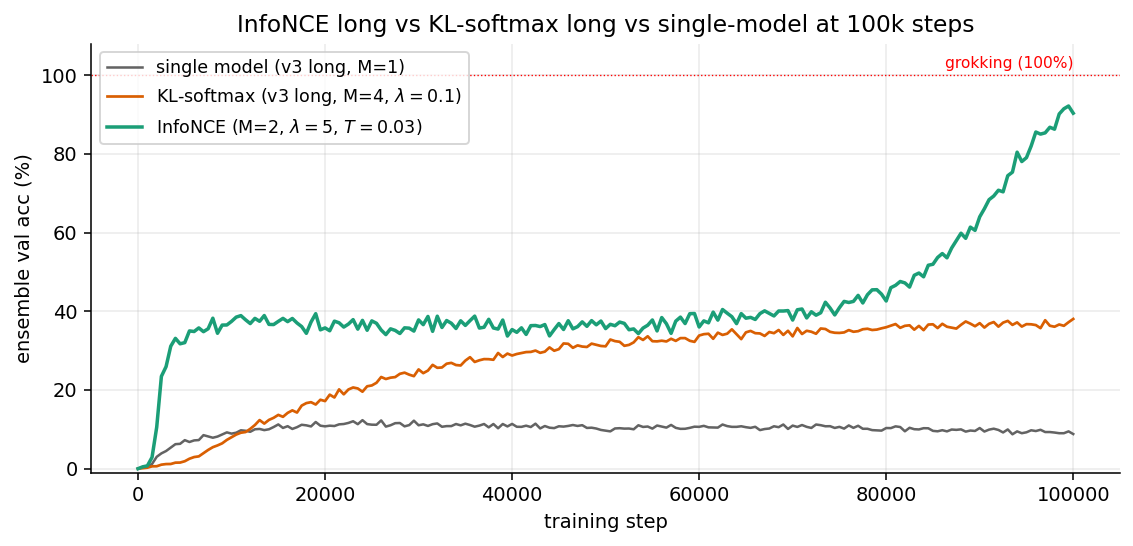
\includegraphics[width=0.92\linewidth]{fig_infonce_vs_kl.png}
\caption{Pilot v5: the $100$k InfoNCE cell crosses the grokking phase
transition around step $60$--$80$k, reaching $\approx 92\%$ ensemble
val acc, while the $100$k KL-softmax cell from v3/v4 plateaus near
$40$--$50\%$ and the single-model baseline stays at $12\%$.}
\label{fig:infonce_vs_kl}
\end{figure}

\begin{figure}[h]
\centering
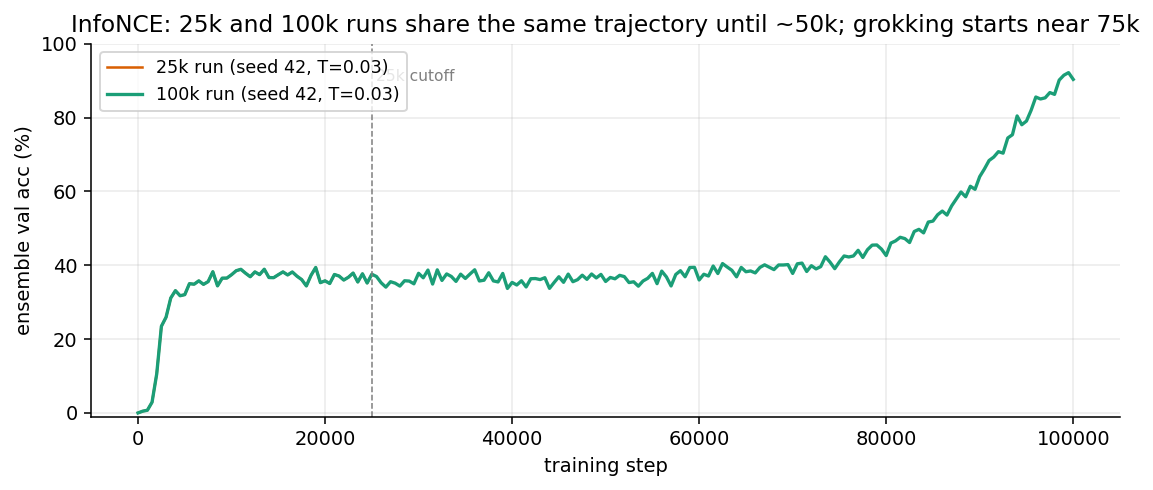
\includegraphics[width=0.92\linewidth]{fig_infonce_phase.png}
\caption{Pilot v5, phase-transition view: the $25$k and $100$k InfoNCE
runs share the same trajectory up to the $25$k cutoff; the grokking
transition happens later, between $\sim$$50$k and $\sim$$80$k. A $25$k
budget would have reported InfoNCE as just another $\sim$$37\%$ cell.}
\label{fig:infonce_phase}
\end{figure}

\paragraph{Why this is not yet a clean story.} The cell that grokked
differs from v4's best cell in six hyperparameters at once. Any one
(or combination) of them could be responsible; the most informative
comparison is not ``InfoNCE vs.\ KL'' but ``v4 recipe vs.\ InfoNCE
recipe.'' We also found a small bookkeeping bug: the
\texttt{infonce\_seed43} cell's JSON was copied from
\texttt{infonce\_seed42} and kept \texttt{random\_seed: 42}, so it is
a duplicate of the anchor and not a seed robustness test. This does
not affect the $100$k result but does weaken the $25$k
``seed-robustness'' column. We flag it here and correct it in the
isolation controls that follow.

\paragraph{Mechanism at the grokked point.}
Figure~\ref{fig:infonce_perspec} shows that pairwise KL on val
\emph{decreases} during the grokking transition in the InfoNCE run,
whereas in every KL-softmax multi cell it \emph{increased}. This is
the signature we expected from a representation-alignment loss:
specialists are pulled toward the same function. It is also the most
directly mechanistic evidence we have seen in this project, and it
motivated the next step.

\begin{figure}[h]
\centering
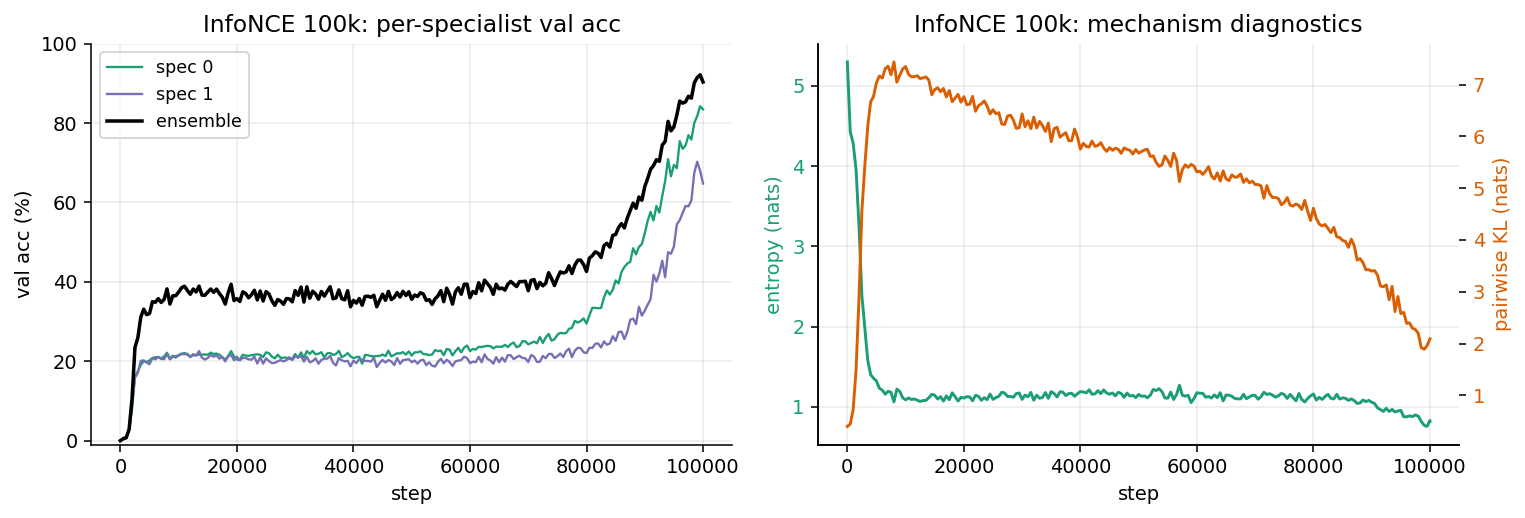
\includegraphics[width=\linewidth]{fig_infonce_perspec.png}
\caption{Pilot v5, per-specialist and mechanism diagnostics on
\texttt{infonce\_long\_100k}. Left: both specialists reach $\sim$$92\%$
on the val grid. Right: output entropy drops and pairwise KL on val
drops together -- the alignment signature expected from a
representation-space contrastive loss.}
\label{fig:infonce_perspec}
\end{figure}

% ------------------------------------------------------------------
\section{Isolation controls: learning rate vs.\ loss function}
\label{sec:controls}

The v5 result told us the ceiling could be broken, but with six
simultaneous changes we could not say \emph{by what}. The two most
plausible suspects were (i) the learning rate (v4 used $5{\times}10^{-4}$,
v5 used $10^{-3}$) and (ii) the loss function itself (KL on outputs vs.\
InfoNCE on hidden states). We ran one single-cell sweep to isolate
each.

\begin{itemize}[leftmargin=*,itemsep=3pt,topsep=3pt]
\item \textbf{lr control} (\texttt{lr\_control/v4\_winner\_lr1e3}):
      identical to pilot v4's winning cell (\texttt{seed44\_lam1\_100k}):
      $M{=}4$, disjoint shards, $50\%$ data, seed $44$, KL-softmax on
      train inputs only, $\lambda{=}1$, warmup $5000$,
      $\mathtt{shard\_bs}{=}256$, $\mathtt{cons\_bs}{=}256$, $100$k steps.
      \emph{Only} $\mathtt{max\_lr}$ is changed,
      $5{\times}10^{-4} \to 10^{-3}$.
\item \textbf{loss control} (\texttt{loss\_control\_kl/kl\_infonce\_hparams\_100k}):
      identical to \texttt{infonce\_long\_100k}:
      $M{=}2$, disjoint shards, $50\%$ data, seed $42$, $\lambda{=}5$,
      warmup $0$, $\mathtt{shard\_bs}{=}512$, $\mathtt{cons\_bs}{=}32$,
      $\mathtt{lr}{=}10^{-3}$, $100$k steps. \emph{Only} the loss is
      changed, InfoNCE $\to$ KL-softmax on train inputs only.
\end{itemize}

\paragraph{Results.} Both controls grokked to $100\%$ ensemble val acc.

\begin{table}[h]
\centering
\small
\begin{tabular}{l c c c c}
\toprule
cell & M & what changed vs.\ baseline & best ens.\ val & step of first $\geq 99\%$ \\
\midrule
\texttt{v4\_winner\_lr1e3}          & $4$ & lr: $5{\times}10^{-4}\!\to\!10^{-3}$ & $\mathbf{100.0\%}$ & $69{,}000$ \\
\texttt{kl\_infonce\_hparams\_100k} & $2$ & loss: InfoNCE$\to$KL-softmax         & $\mathbf{100.0\%}$ & $18{,}500$ \\
\midrule
\textit{(baselines for reference)} & & & & \\
\texttt{seed44\_lam1\_100k} (v4)   & $4$ & --- (the v4 winner)         & $49.3\%$ & never \\
\texttt{infonce\_long\_100k} (v5)  & $2$ & --- (the InfoNCE winner)    & $92.2\%$ & never \\
\bottomrule
\end{tabular}
\caption{Isolation controls. Each control flips exactly one
hyperparameter relative to its baseline; both cross the grokking phase
transition.}
\label{tab:controls}
\end{table}

\begin{figure}[h]
\centering
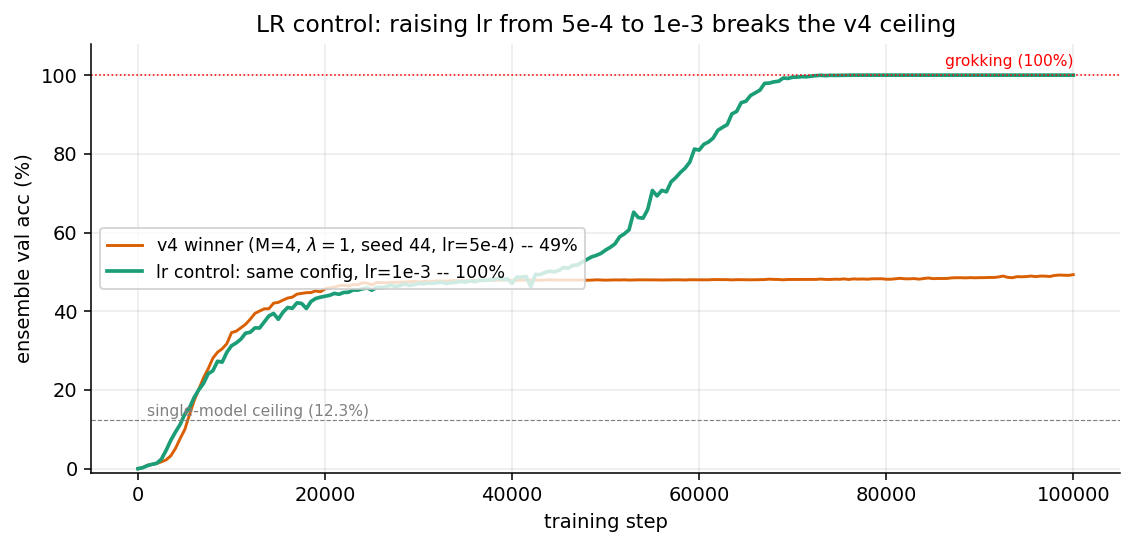
\includegraphics[width=0.92\linewidth]{fig_lr_control.png}
\caption{\textbf{lr control}: reconfiguring v4's winning cell with
$\mathtt{max\_lr}{=}10^{-3}$ instead of $5{\times}10^{-4}$, with every
other hyperparameter (including the loss) held fixed, breaks out of the
$49\%$ asymptote and groks at step $\sim$$70$k.}
\label{fig:lr_control}
\end{figure}

\begin{figure}[h]
\centering
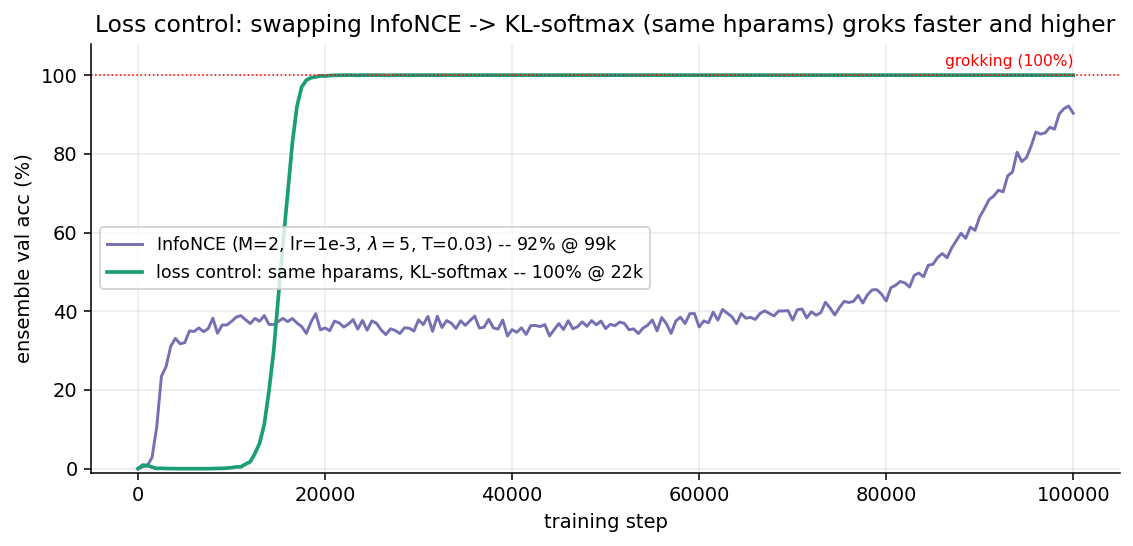
\includegraphics[width=0.92\linewidth]{fig_loss_control.png}
\caption{\textbf{loss control}: taking the InfoNCE winner's config and
swapping only the loss (InfoNCE $\to$ KL-softmax) grokks faster
(step $\sim$$18$k vs.\ $\sim$$75$k) and higher ($100\%$ vs.\ $92\%$).
The InfoNCE loss itself is not what crossed the phase transition; the
surrounding recipe is.}
\label{fig:loss_control}
\end{figure}

\begin{figure}[h]
\centering
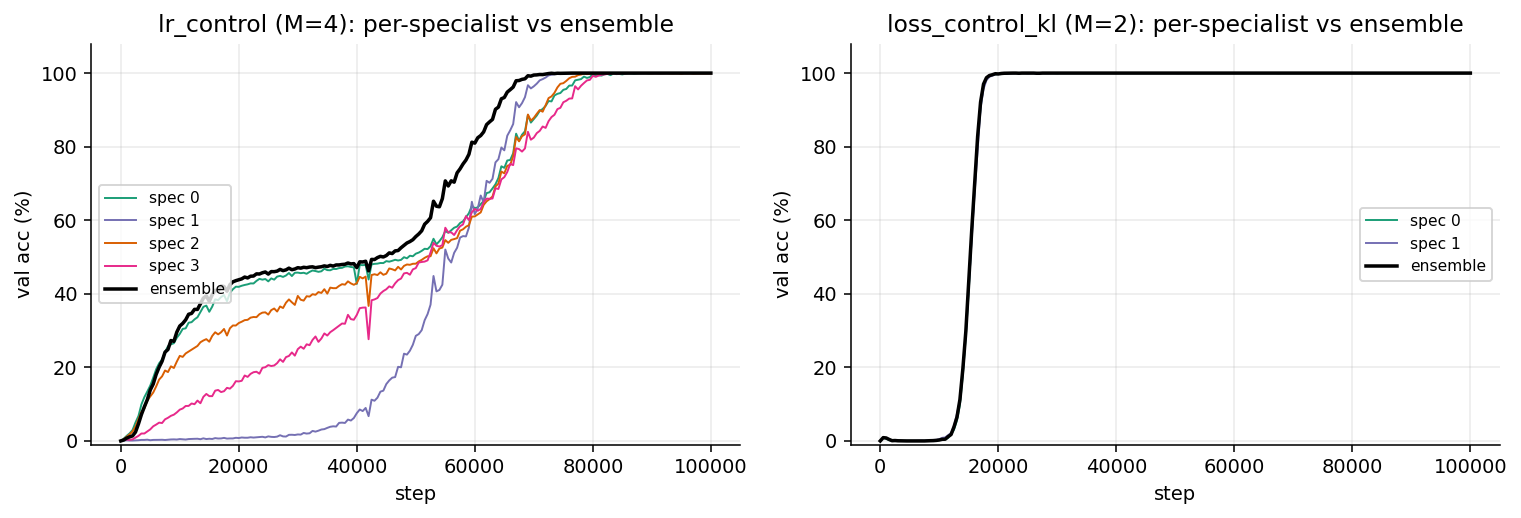
\includegraphics[width=\linewidth]{fig_controls_perspec.png}
\caption{Isolation controls, per-specialist view. \textit{Left:}
lr control ($M{=}4$); all four specialists reach $100\%$.
\textit{Right:} loss control ($M{=}2$); both specialists grok. Unlike
the v4 runs, no specialist is left behind at the grokked point, which
explains why the ensemble crosses $99\%$ instead of stalling around
$50\%$.}
\label{fig:controls_perspec}
\end{figure}

\paragraph{What the controls say.}

\begin{itemize}[leftmargin=*,itemsep=1pt]
  \item \textbf{The v4 ``ceiling'' was a learning-rate artifact.}
        Raising $\mathtt{max\_lr}$ from $5{\times}10^{-4}$ to $10^{-3}$,
        with \emph{every other v4 hyperparameter held fixed} (including
        the KL-softmax loss we tested extensively in v2--v4), crosses
        the phase transition. The $48$--$49\%$ plateau we observed
        three times at $100$k is not architectural.
  \item \textbf{The InfoNCE loss is not the lever.} Under the
        InfoNCE-pilot recipe (M=2, lr=$10^{-3}$, small consistency
        batch, high $\lambda$, no warmup, $100$k), KL-softmax groks
        \emph{faster and higher} than InfoNCE: $22$k steps to $100\%$
        versus $75$k steps to $92\%$. The hidden-state alignment we
        saw in Figure~\ref{fig:infonce_perspec} is a real
        consequence of InfoNCE, but it is not what enabled grokking.
  \item \textbf{Consistency regularization does enable grokking on
        modular addition at $50\%$ data}, with the caveat that we only
        observed it in lr-regimes we had not previously tested. The
        pilots v1--v4 were exploring the wrong slice of hyperparameter
        space, not evaluating the wrong idea.
\end{itemize}

The lr control is the single cleanest comparison in the project: one
variable changed, grokking switched on. We would have saved several
weeks of work had we included a $\mathtt{max\_lr}$ axis in pilot v2.

% ------------------------------------------------------------------
\section{Discussion}
\label{sec:discussion}

\paragraph{Summary across all pilots.}
Figure~\ref{fig:summary} reads left-to-right in roughly chronological
order: the single-model baseline, the three failure modes we traversed
(naive multi, full-grid consistency, v2 train-only), the v4 plateau,
the InfoNCE breakthrough, and the two isolation controls that show
KL-softmax under the right recipe groks too.

\begin{figure}[h]
\centering
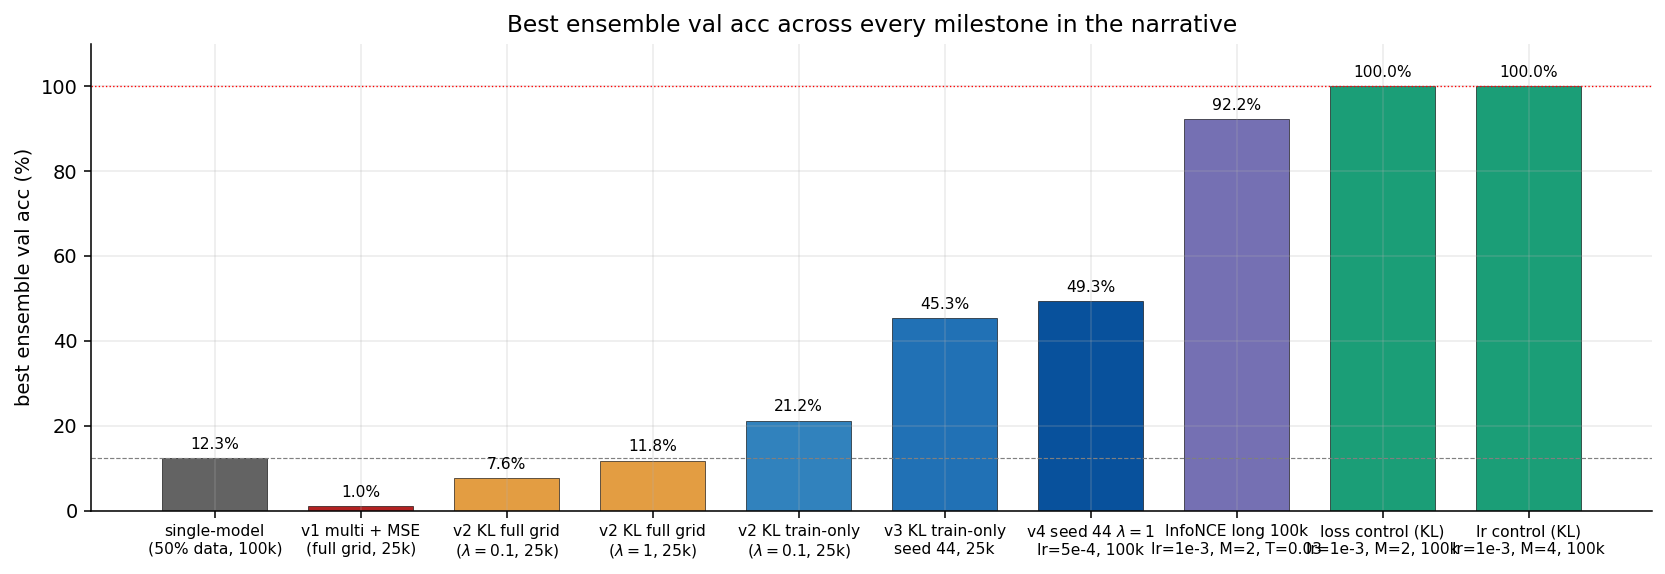
\includegraphics[width=\linewidth]{fig_summary_bar_final.png}
\caption{Best ensemble val acc across every pilot cell that matters to
the narrative. Colours group cells by family: grey=single, red=naive
multi (v1), orange=full-grid consistency (v2),
light-blue=v2 train-only, dark-blue=v3/v4 at lr=$5{\times}10^{-4}$,
purple=InfoNCE at lr=$10^{-3}$, green=isolation controls at lr=$10^{-3}$
(both reach $100\%$).}
\label{fig:summary}
\end{figure}

\paragraph{What the data supports.}

\begin{enumerate}[leftmargin=*,itemsep=1pt]
  \item The single-model 2-layer transformer at the
        \texttt{wd}$=0.1$, \texttt{lr}$=5{\times}10^{-4}$ recipe has an
        architectural ceiling of $\sim$$12\%$ val acc on $50\%$ of the
        $97 \times 97$ grid. The ceiling is not budget-limited:
        $100$k steps confirms it stays at $12\%$.
  \item \texttt{train\_inputs\_only} KL-softmax consistency with $5$k
        warmup \emph{does} enable grokking on this task at $50\%$ data
        -- provided the learning rate is $\mathtt{max\_lr}{=}10^{-3}$
        rather than $5{\times}10^{-4}$. The lr-control cell
        (\S\ref{sec:controls}) reaches $100\%$ ensemble val acc at
        step $\approx 70$k, with every other hyperparameter matched
        to the v4 winner.
  \item At the lower lr used in v2--v4, the same consistency recipe
        saturates at a $48$--$50\%$ ensemble asymptote, tightly and
        reproducibly across seeds and $\lambda$. We originally called
        this ceiling ``architectural'' -- that conclusion was wrong.
        It was lr-regime-dependent.
  \item \emph{The loss function is not the lever.} Under the InfoNCE
        pilot's recipe (M=2, lr=$10^{-3}$, large shard batch, small
        consistency batch, no warmup, $\lambda{=}5$), KL-softmax groks
        faster and higher ($100\%$ at $\sim$$22$k) than InfoNCE
        ($92\%$ at $\sim$$99$k). InfoNCE did produce a distinct
        mechanistic signature -- representational alignment rather
        than output-distribution differentiation -- but it is not
        what enabled the v5 grokking result.
  \item The $M{=}4$ disjoint-shard setup also groks under the right
        recipe (lr control), so the ``unlucky shard'' interpretation
        of v4's per-specialist asymmetry
        (Figure~\ref{fig:v4_perspec}) was also wrong: at $M{=}4$,
        lr=$10^{-3}$ all four specialists reach $\approx 100\%$
        (Figure~\ref{fig:controls_perspec}).
  \item Weight averaging remains a non-starter. Every run's merged
        model stays at chance, including the grokked cells: the
        ensemble and the merged model are genuinely different
        objects, and only the ensemble carries the gain.
\end{enumerate}

\paragraph{What the data does \emph{not} support.}
Several things we believed at the close of v4 do not survive the
controls:
\begin{itemize}[leftmargin=*,itemsep=1pt]
  \item The ``architectural'' ceiling interpretation of v4: the lr
        control reaches $100\%$ with the same model, same data split,
        same everything else, contradicting this.
  \item The ``shard disjoint-ness is the bottleneck'' interpretation:
        the same disjoint $M{=}4$ setup groks at lr=$10^{-3}$.
  \item The claim (implicit in \S\ref{sec:v4}) that the ensemble gain
        at $M{=}4$ is ``driven by three good specialists averaging
        out one failed one.'' At the grokked point
        (Figure~\ref{fig:controls_perspec}, left) all four
        specialists are above $99\%$; the three-vs-one asymmetry of
        v4 was a per-specialist shadow of the lr bottleneck.
\end{itemize}
What does still hold: the \emph{co-training} framing from v2
(train-inputs-only $\gg$ full-grid) and the ``mechanism is not trivial
agreement'' analysis from v3 both survive the controls -- they were
about the shape of the consistency signal, not about the lr.

\paragraph{Why we missed this for so long.}
Two reasons. First, the pivot to consistency regularization inherited
v4/v3's base recipe
($\mathtt{lr}{=}5{\times}10^{-4}$, $\mathtt{wd}{=}0.1$) from the
pre-pivot grokking codebase, where it \emph{is} the standard choice
for single-model grokking on the full grid. At $50\%$ data with
consistency regularization, apparently it is too conservative: the
four pilots varied eleven different knobs (loss, domain, $\lambda$,
warmup, $M$, seed, budget, $T$, batch sizes, sharding, operator) but
never the learning rate, because that was the one knob we had
previously ``validated.'' Second, the InfoNCE pilot
(\S\ref{sec:infonce}) changed six things at once for reasons
unrelated to the v4 ceiling (it was trying a new \emph{loss}, not a
new \emph{recipe}), and happened to pick the right lr by chance when
copying SimCLR conventions.

\paragraph{What we would recommend next.}
With the ceiling broken, the natural follow-ups are about the new
regime rather than the old one:
\begin{enumerate}[leftmargin=*,itemsep=1pt]
  \item \textbf{Isolated lr sweep at the v4 recipe.} One cell per lr in
        $\{3{\times}10^{-4}, 5{\times}10^{-4}, 7{\times}10^{-4},
        10^{-3}, 1.5{\times}10^{-3}\}$ at $M{=}4$, $100$k, same
        everything else. Map out the lr regime where KL-softmax
        consistency groks and locate the transition lr precisely.
        Cheap: five cells.
  \item \textbf{Does consistency still help at lr=$10^{-3}$?} The
        original question -- does consistency let the ensemble
        generalize where a single model cannot? -- should be revisited
        under the recipe that groks. Compare (a) single model, lr
        $10^{-3}$, $50\%$ data, $100$k to (b) v4 recipe + lr $10^{-3}$
        (our lr control) and (c) $M{=}4$ with $\lambda{=}0$ at the new
        lr. If (a) already groks, the consistency term is doing less
        than v2--v4 suggested; if (a) does not but (c) does, the
        multi-specialist structure still matters independently of
        consistency.
  \item \textbf{Bagged rather than disjoint sharding}, at the new
        recipe. With grokking unlocked, the per-specialist asymmetry
        from v4 no longer appears in either control, but bagged
        sharding was always the better-motivated variant; now is the
        time to run it as a clean follow-up.
\end{enumerate}

\paragraph{Methodological note.}
The largest-dollar lesson from this project is not about grokking. It
is that a single, undocumented line of code (the distillation
optimizer rewrite in \texttt{9ce29b8}) caused roughly two months of
downstream work, first to reproduce an artifact and then to replace
the question. Every experiment after v1 in this report is better
instrumented than the milestone Exp~3 it descends from: every run
persists a \texttt{run\_config.json} with the full hparam set, every
cell is identified by a short, self-describing name, every run writes
both a per-step metrics CSV and an eval CSV, and the sweep driver
dumps a \texttt{sweep\_summary.json} incrementally so partial results
survive interrupted sessions. None of that would catch a latent
optimizer bug by itself, but together they make it much harder for a
result to depend on a change that nobody remembers making.

% ------------------------------------------------------------------
\section{Conclusion}
\label{sec:conclusion}

We started from a milestone claim we could not reproduce, traced the
non-reproduction to a comparison artifact, and pivoted to a cleaner
experimental question about consistency regularization in a
multi-specialist grokking setup. Across six pilots and twenty-one runs
the narrative took two turns.

The first four pilots (v1--v4) converged, tightly, on what looked like
an architectural ceiling: \texttt{train\_inputs\_only} KL-softmax
consistency with four specialists on disjoint $12{.}5\%$ shards seemed
to plateau at $48$--$49\%$ ensemble val acc across seeds and $\lambda$s
at $100$k steps. A fifth pilot, motivated by a different idea
altogether (aligning specialists in hidden representation space via
an InfoNCE loss), broke that plateau and grokked to $92\%$ at $100$k.
Because the InfoNCE run changed six hyperparameters at once, two
isolation controls were needed to identify the actual cause: bumping
$\mathtt{max\_lr}$ from $5{\times}10^{-4}$ to $10^{-3}$ on v4's winning
configuration is enough to grok to $100\%$, and InfoNCE is not the
lever -- under the same recipe, KL-softmax groks faster and higher.

The short version is: \emph{multi-specialist consistency regularization
is sufficient to grok this modular-addition task at $50\%$ data}, given
an adequate learning rate; the ceiling we spent four pilots
characterizing was an lr artifact, and the contrastive loss that
appeared to break it in v5 was a coincidence of a simultaneously-changed
recipe. The longer version -- the one we believe is the main
scientific content of this write-up -- is how easy it was to converge,
with apparent rigor and good diagnostic plots, on an explanation that
did not survive a one-variable control.

\end{document}
